%%%%%%%%%%%%%%%%%%%%%%%%%%%%%%%%%%%%%%%%%%%%%%%%%%%%%%%%
\documentclass[10pt, aspectratio=169]{beamer}
\usepackage[many]{tcolorbox}
\usetheme{metropolis}
\usepackage[english]{babel}
\usepackage[utf8]{inputenc}
\usepackage[T1]{fontenc}
\usepackage{array}
\usepackage{booktabs}
\usepackage{colortbl}
\usepackage{multirow}
\usepackage{graphicx}
\usepackage{mathrsfs}
\usepackage{bbding}
\usepackage{pifont}
\usepackage{wasysym}
\usepackage{amssymb}
\usepackage{enumerate}
\usepackage{booktabs,threeparttable}
\usepackage{adjustbox}
\usepackage{tikz}
\usetikzlibrary{calc}
\usepackage{geometry}
\usepackage{appendixnumberbeamer}


% DEFINE COLORPALETTE
\newcommand{\cmark}{\ding{51}}%
\newcommand{\xmark}{\ding{55}}
\definecolor{unibasmintlight}{RGB}{233, 255, 253}
\definecolor{unibasmint}{RGB}{165,215,210}
\definecolor{unibasmintmid}{RGB}{30,165,165}
\definecolor{unibasanthr}{RGB}{45,55,60}
\definecolor{unibasgreydark}{RGB}{140,145,150}
\definecolor{unibasred}{RGB}{210,5,55}
\definecolor{unibaspink}{RGB}{235,130,155}
\definecolor{unibasgrey}{RGB}{190,195,200}
\definecolor{unibasmintdark}{RGB}{0,110,110}
\definecolor{unibasblack}{RGB}{0,0,0}
\definecolor{unibaswhite}{RGB}{255,255,255}

\definecolor{scenA_table}{RGB}{245, 245, 180}
\definecolor{scenB_table}{RGB}{235, 215, 245}
\definecolor{scenC_table}{RGB}{200, 225, 240}

\definecolor{capacity_upgrade}{RGB}{64, 153, 153}
\definecolor{capacity_expansion}{RGB}{162, 216, 216}


% -------------------------------------------------------
% METROPOLIS COLOR SETUP
% -------------------------------------------------------
% \setbeamercolor{normal text}{fg=unibasanthr, bg=white}
% \setbeamercolor{alerted text}{fg=unibasred}
% \setbeamercolor{example text}{fg=unibasmintdark}

% \setbeamercolor{frametitle}{bg=unibasmintlight, fg=unibasmintdark}
% \setbeamercolor{title separator}{fg=unibasmintdark}
% \setbeamercolor{progress bar}{fg=unibasmintdark, bg=unibasgrey}

% \setbeamercolor{block title}{bg=unibasmintdark, fg=unibasmint}
% \setbeamercolor{block body}{bg=unibasmintlight, fg=unibasanthr}
% \setbeamercolor{block title alerted}{bg=unibasred, fg=white}
% \setbeamercolor{block body alerted}{bg=unibasmintlight!50, fg=unibasanthr}

% \setbeamercolor{title}{fg=unibasmintdark}
% \setbeamercolor{subtitle}{fg=unibasgreydark}
% \setbeamercolor{author}{fg=unibasanthr}
% \setbeamercolor{institute}{fg=unibasgreydark}
% \setbeamercolor{date}{fg=unibasgreydark}

% \setbeamercolor{section in toc}{fg=unibasmintdark}
% \setbeamercolor{subsection in toc}{fg=unibasgreydark}

% \setbeamercolor{itemize item}{fg=unibasmintdark}
% \setbeamercolor{itemize subitem}{fg=unibasmintmid}
% \setbeamercolor{itemize subsubitem}{fg=unibasgreydark}
% \setbeamercolor{enumerate item}{fg=unibasmintdark}

% \setbeamercolor{button}{bg=unibasmint, fg=unibasanthr}

% footer / standout
\setbeamercolor{footline}{fg=unibasgreydark, bg=white}

% -------------------------------------------------------
% METROPOLIS FONT / STYLE OPTIONS
% -------------------------------------------------------
\metroset{
  titleformat        = regular,
  titleformat frame  = regular,
  sectionpage        = none,
  numbering          = fraction,
  progressbar        = frametitle,
  block              = fill
}

\usefonttheme[onlymath]{serif}
\setbeamertemplate{caption}[numbered]


% % -------------------------------------------------------
% % BLOCK ENVIRONMENT COLORS (inside block/alertblock)
% % -------------------------------------------------------
% \AtBeginEnvironment{block}{%
%   \setbeamercolor{itemize item}{fg=unibasmintdark}
%   \setbeamercolor{itemize subitem}{fg=unibasmintmid}
%   \setbeamercolor{enumerate item}{fg=unibasmintdark}
%   \setbeamercolor{item projected}{fg=white, bg=unibasmintdark}
% }

% \AtBeginEnvironment{alertblock}{%
%   \setbeamercolor{itemize item}{fg=unibasred}
%   \setbeamercolor{enumerate item}{fg=unibasred}
%   \setbeamercolor{item projected}{fg=white, bg=unibasred}
% }

% -------------------------------------------------------
% CITATIONS
% -------------------------------------------------------
\usepackage[backend=biber, style=apa, maxbibnames=999, minbibnames=1,
            maxcitenames=1, mincitenames=1, uniquelist=true]{biblatex}
\addbibresource{optimalpv_conf.bib}
\AtBeginBibliography{\small}
% \hypersetup{colorlinks=true,
%             citecolor=unibasmintmid,
%             linkcolor=unibasmintdark,
%             urlcolor=unibasmintdark}

% -------------------------------------------------------
% BACKUP FRAME COUNTER
% -------------------------------------------------------
\newcommand{\backupbegin}{
  \newcounter{framenumberappendix}
  \setcounter{framenumberappendix}{\value{framenumber}}
}
\newcommand{\backupend}{
  \addtocounter{framenumberappendix}{-\value{framenumber}}
  \addtocounter{framenumber}{\value{framenumberappendix}}
}

% -------------------------------------------------------
% TITLE INFO
% -------------------------------------------------------
% \title[Improved Residential PV Expansion]{Decisions at the Grid's Edge}
\title{Update Primeo}
\subtitle{Decisions at the Grid's Edge - An Improved Spatial PV Expansion in Swiss Residences}
\author{Raul Hochuli (raul.hochuli@unibas.ch)}
\institute{Universität Basel, Wirtschaftswissenschaftliche Fakultät}
\date{Juni 2026}
% \titlegraphic{\includegraphics[width=2.3cm]{UniBas_Logo.jpg}}


%*******************************************************************************
\begin{document}
%*******************************************************************************

% -------------------------------------------------------
\begin{frame}
  \maketitle
\end{frame}


%%%%%%%%%%%%%%%%%%%%%%%%%%%%%%%%%%%%%%%%%%%%%%%
\section{Adjustments to last Presentation}

% -------------------------------------------------------
\begin{frame}{Übersicht Anpassungen}
\begin{enumerate}

    \item \textbf{Unrealistische Ausbaukapazität}  \hyperlink{adjusted_res_capacity}{\beamergotobutton{ Angepasste Ausbaukazapität}}
    \begin{itemize}
        \item Bisher: Zukünftiger PV Ausbaupfad gemäss Energieperspektive 2050+ (EP2050+) als unrealistische Annahme. 
        \item \textit{
            Neu: Startwert basiert auf historischem Wert (2023), anschliessend asymptotische Annäherung an die Zielkapazität EP2050+ bis 2050. 
            }
    \end{itemize}
    %
    \textbf{\item Batteriespeicher gegen Überproduktion} \hyperlink{worstnodesworstweek}{\beamergotobutton{ Überproduktion: Schlimmster Tag in den schlimmsten Trafos}}
    \begin{itemize}
        \item Bisher: Batteriespeicher wird im Model nicht berücksichtigt (bestehend + zukünftig) aufgrund fehlender Datenquellen und strengen Annahmen zum Ladeverhalten. 
        \item \textit{
            % Neu: Vergleich von Überproduktion in den schlimmsten Kontenpunkten zu herkömlicher Speicherkapazität. 
            Neu: Herkömmlicher Speicher könnte eine 24h Überproduktion evtl. auffangen, jedoch bis zum nächsten Tag nicht genügend entladen. 
            }
        % Post-Analyse: Batteriespeicher in den "schlimmsten" Kontenpunkten
        % Erwartungsgemäss erfolgt der grösste Teil der Überproduktion (aufgrund von Trafokapazität nicht aufnehmbar) an einem Sommertag in Netzbereichen mit vielen Häuser. 
        % }
        % \item \textit{
        % Am Ende der Simulation, also bei maximaler Installationsrate, entfallen am "schlimmsten" Tag ca. 15-20 kWh pro Haus in den 5 meist betroffenen Knotenpunkten. Dies könnte mit herkömlichem Heimspeicher zu grossen Teilen aufgefangen werden, das Problem wäre aber ncht genügend die Entladung in den Abend / Morgenzeiten in diesen Tagen. 
        % }
    \end{itemize}
    %
    \item \textbf{Effekte von Preisänderungen (Strompreis)} \hyperlink{npv_hists_elecpri}{\beamergotobutton{ Sensitivitätsanalyse: Halbierung / Verdoppelung Strompreis}}
    \begin{itemize}
        \item Bisher: Strompreise und Einspeisetarife bleiben fix über die ganze Simulation. 
        \item \textit{
        Zusätzliche Sensitivitätsanaylse: Erhöhung des Strompreiswas verschiebt die Nullgrenze des NPV-Histogramm, sodass in der Simulation mehr Installationen verbaut werden. Anlagen mit hohem Eigenverbrauchsanteil werden in der Reihenfolge weiter nach vorne geschoben. 
        }
    % : Nur profitable Installationen werden verbautUnprofitable Häuser (mit negativem NPV) erhielten trotzdem eine PV Installation, wenn auch ganz am Schluss der Simulation
    %     \item \textit{
    %     Neu: Nur Häuser mit positivem NPV entscheiden sich für eine Installation. Subentionen des Papers (ABC) haben jetzt Einfluss auf die Installationsreihenfolge \textbf{und} Installationsmenge (bspw. auch Status Quo vs. Abschaffung KEV). 
    %     }
    %     \item \textit{
    %     Sensitivitätsanaylse: Bspw. Senkung des Strompreises in der Zukunft würde  ändert die Mhätten
    %     }
    \end{itemize}
\end{enumerate}
\end{frame}

%%%%%%%%%%%%%%%%%%%%%%%%%%%%%%%%%%%%%%%%%%%%%%%
\section{Results}

% % -------------------------------------------------------
% \begin{frame}{Adjusted Future Installation Capacity}
% \begin{minipage}{0.48\textwidth}
%   \centering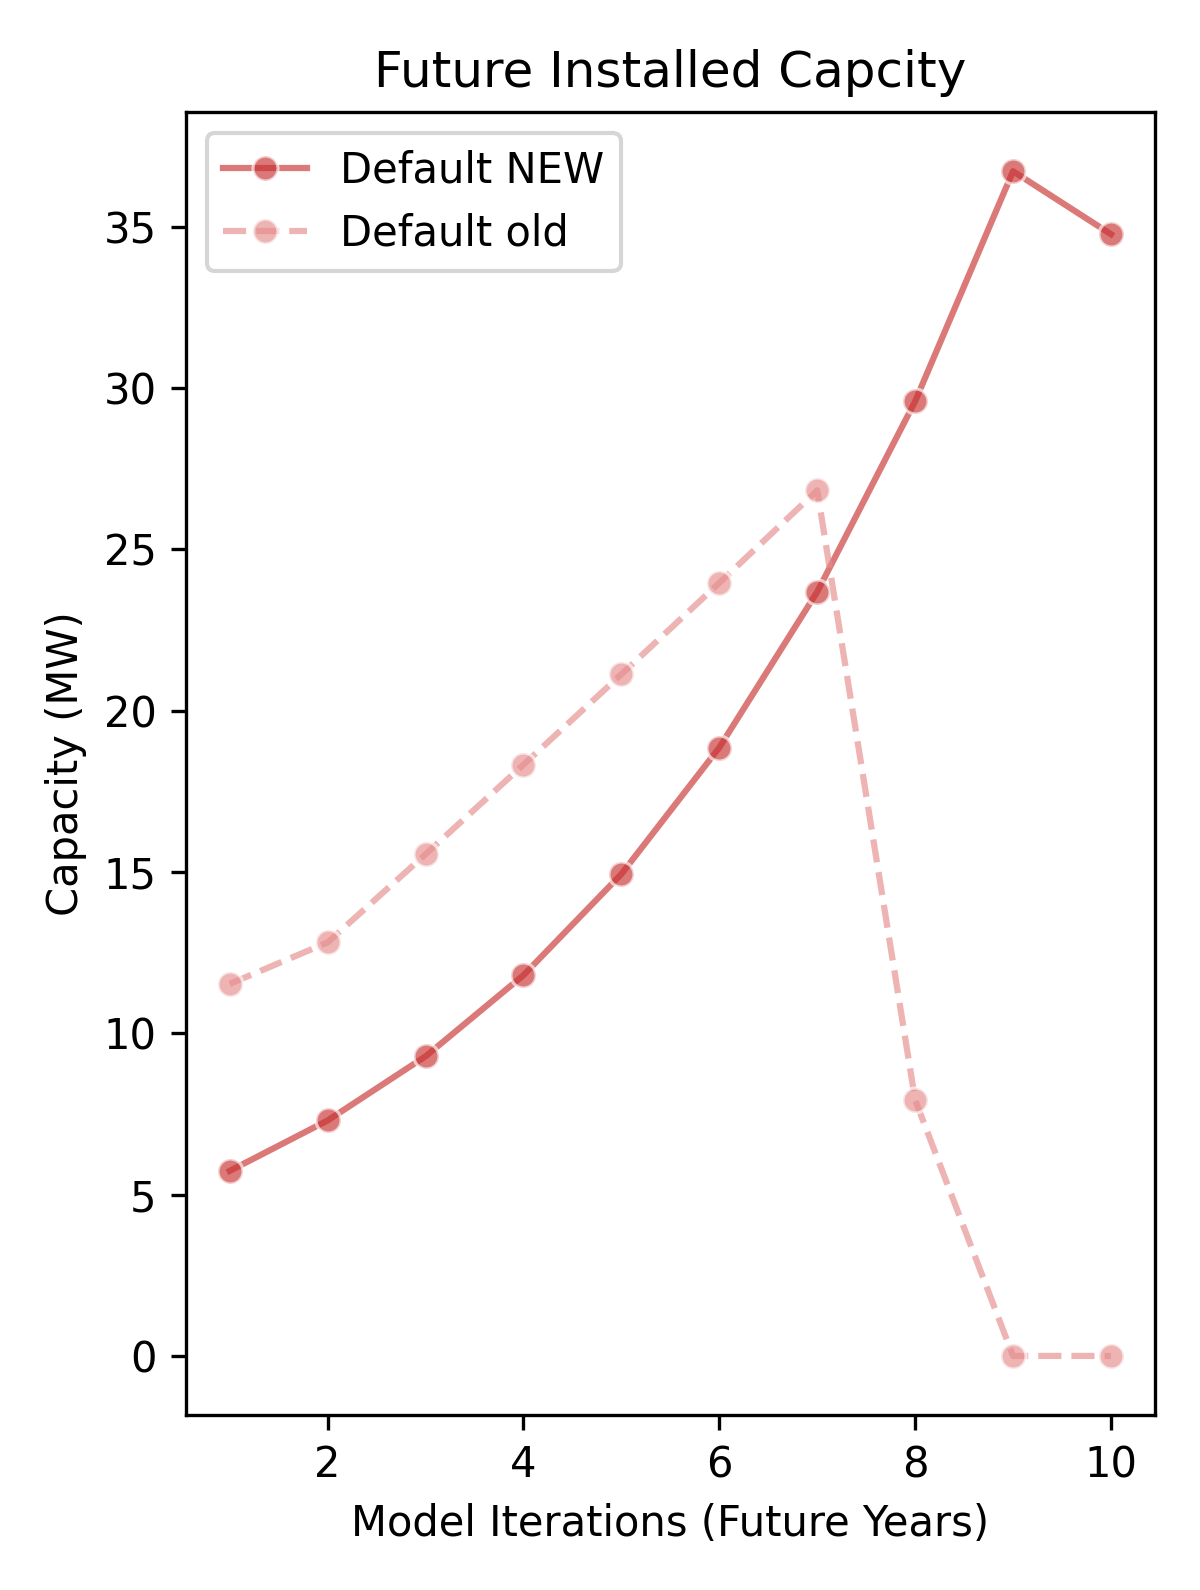
\includegraphics[width=\textwidth]{figures/line_PVproduction_instCap1.png}
% \end{minipage}\hfill
% \begin{minipage}{0.48\textwidth}
%   \centering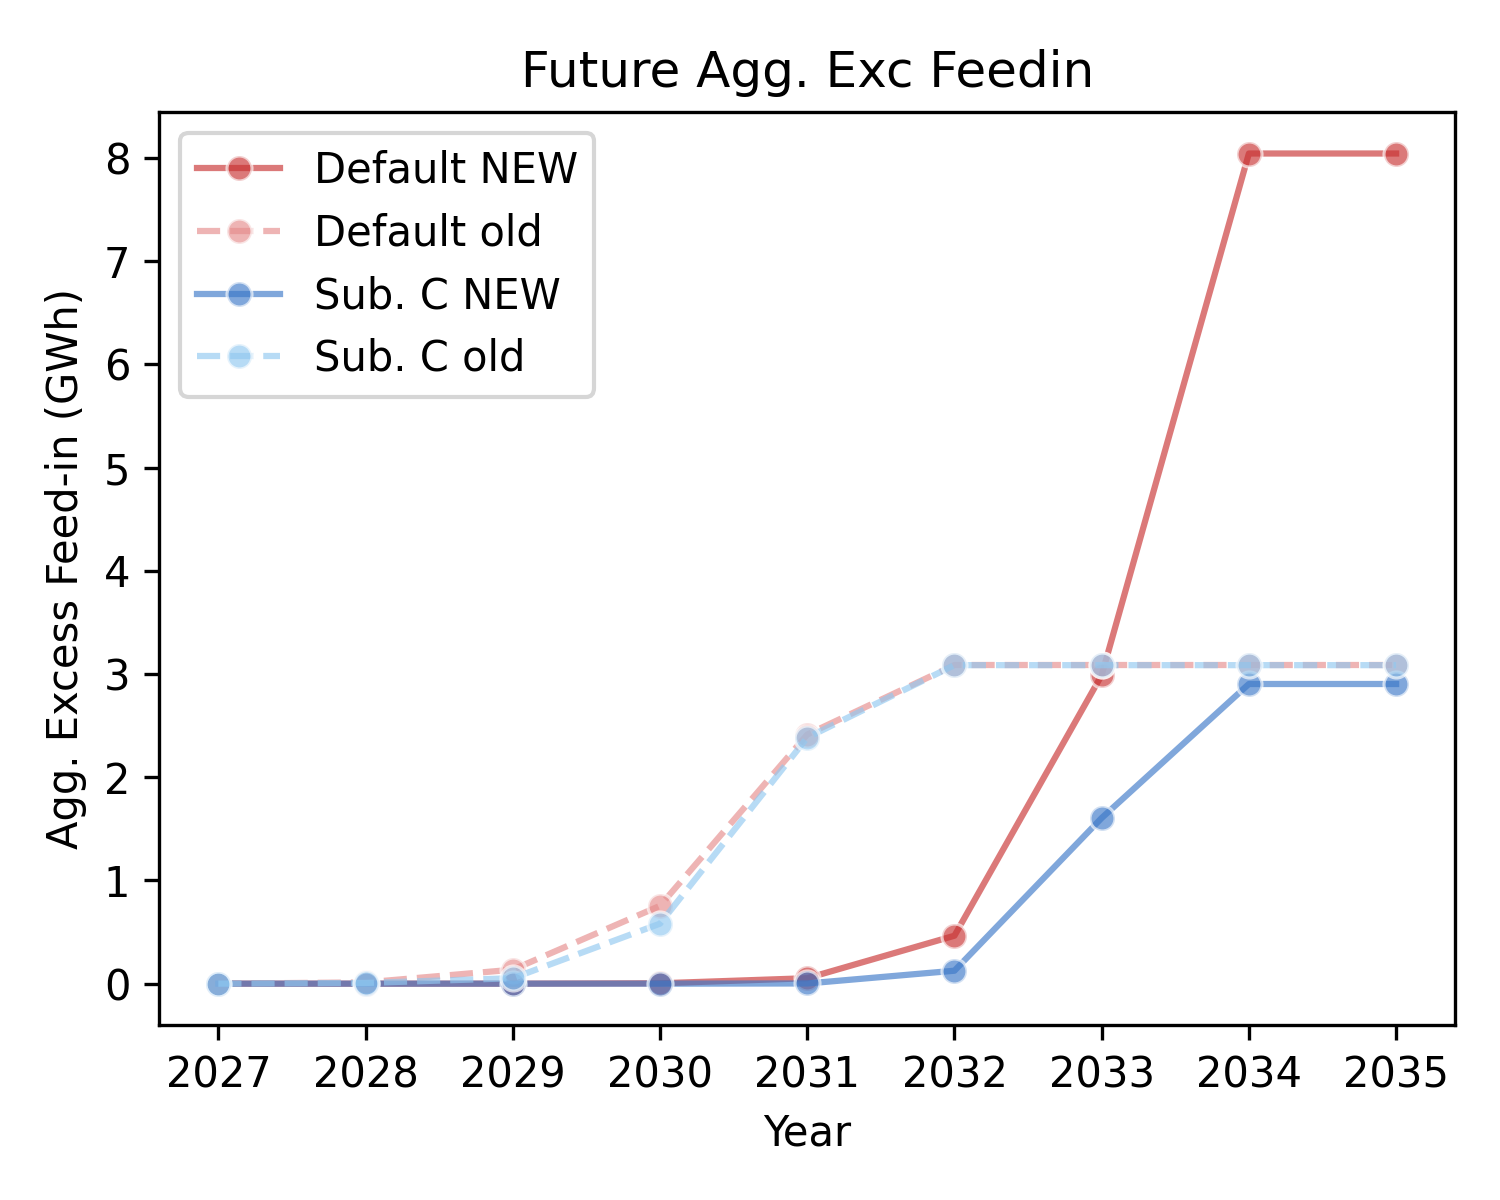
\includegraphics[width=\textwidth]{figures/line_PVproduction_excfeedin1.png}
% \end{minipage}
% \end{frame}



% -------------------------------------------------------
\begin{frame}[t]{Angepasste Ausbaukazapität}
\hypertarget{adjusted_res_capacity}{}   

\begin{minipage}{0.322\textwidth}
  \centering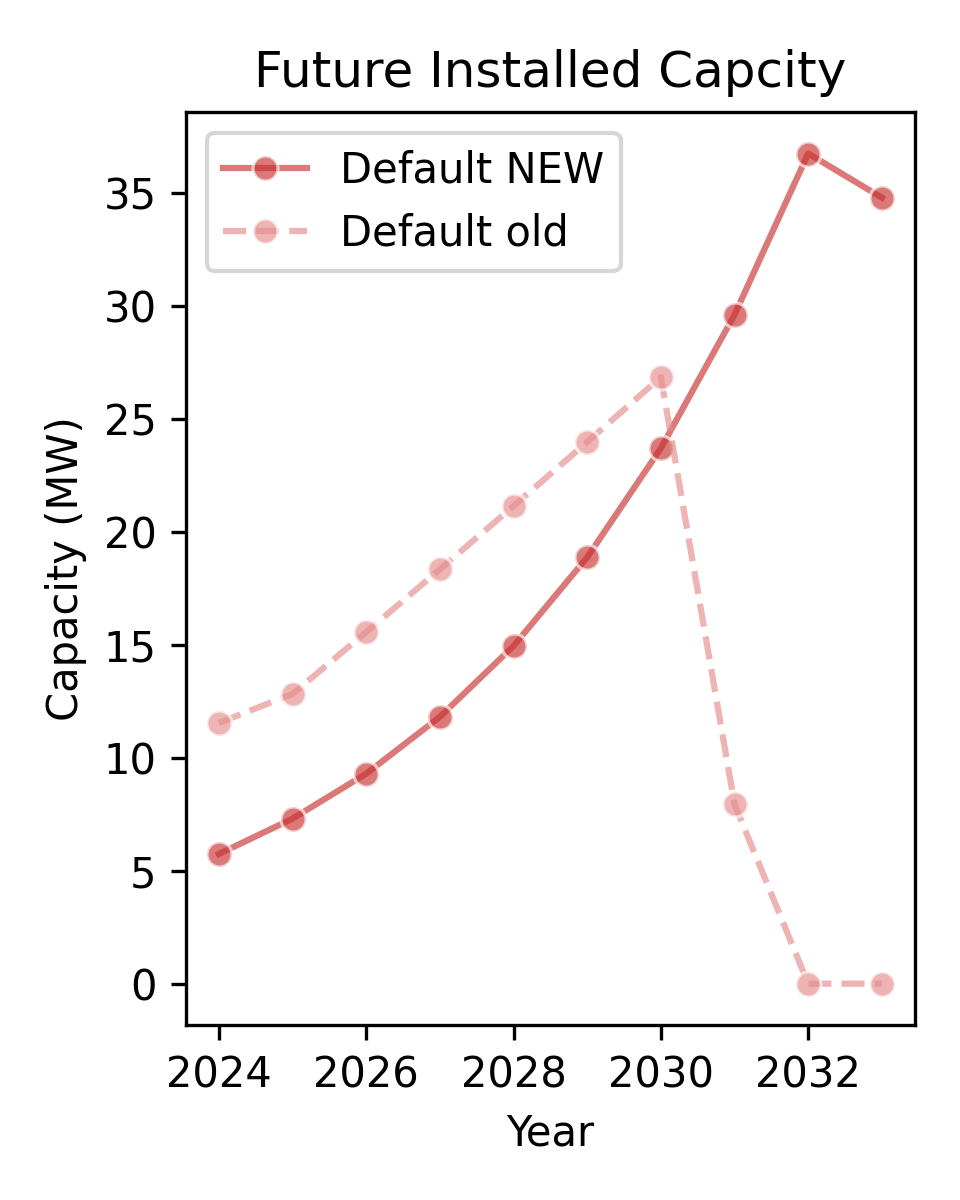
\includegraphics[width=\textwidth]{figures/line_PVproduction_instCap2.png}
\end{minipage}\hfill
\begin{minipage}{0.322\textwidth}
  \centering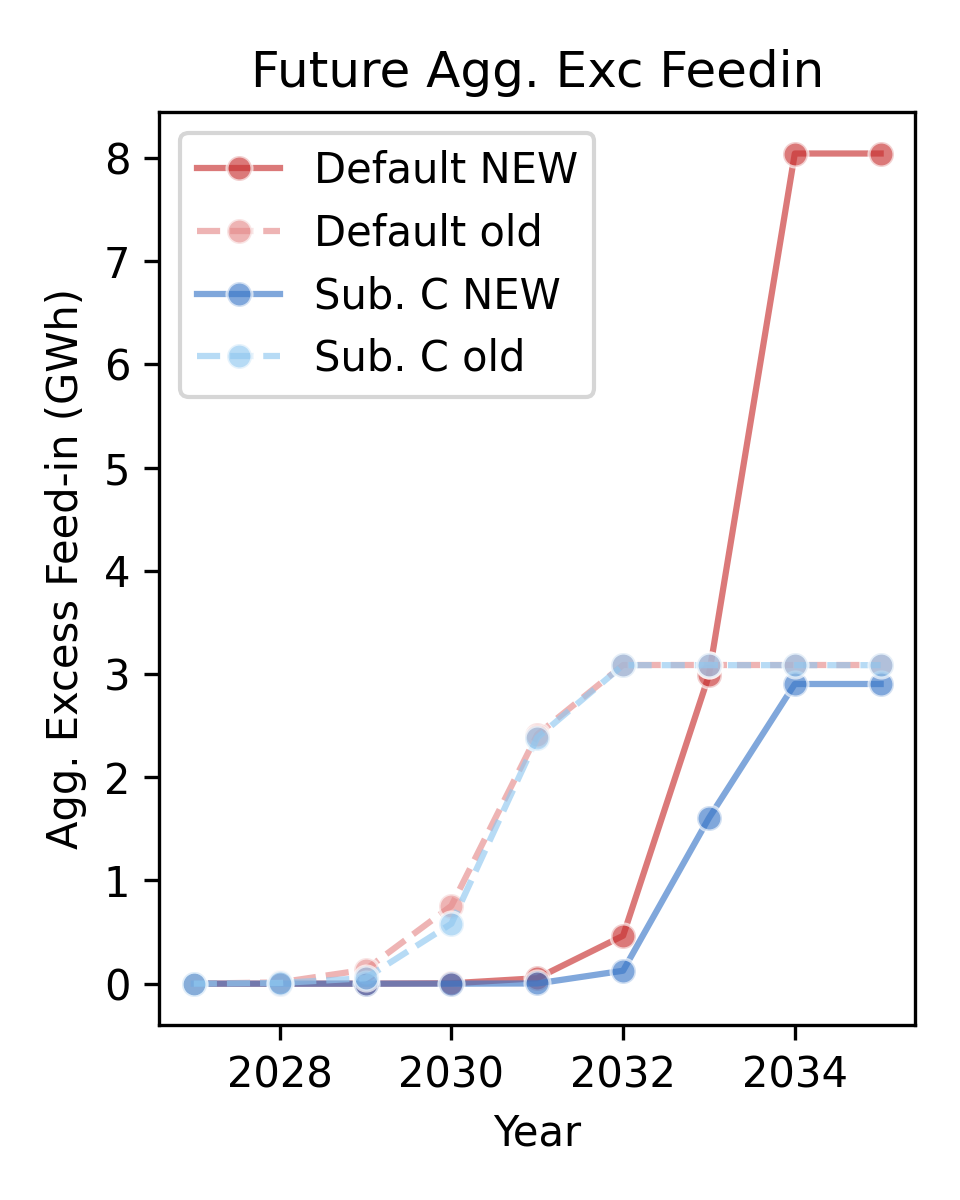
\includegraphics[width=\textwidth]{figures/line_PVproduction_excfeedin2.png}
\end{minipage}\hfill
\begin{minipage}{0.322\textwidth}
  \centering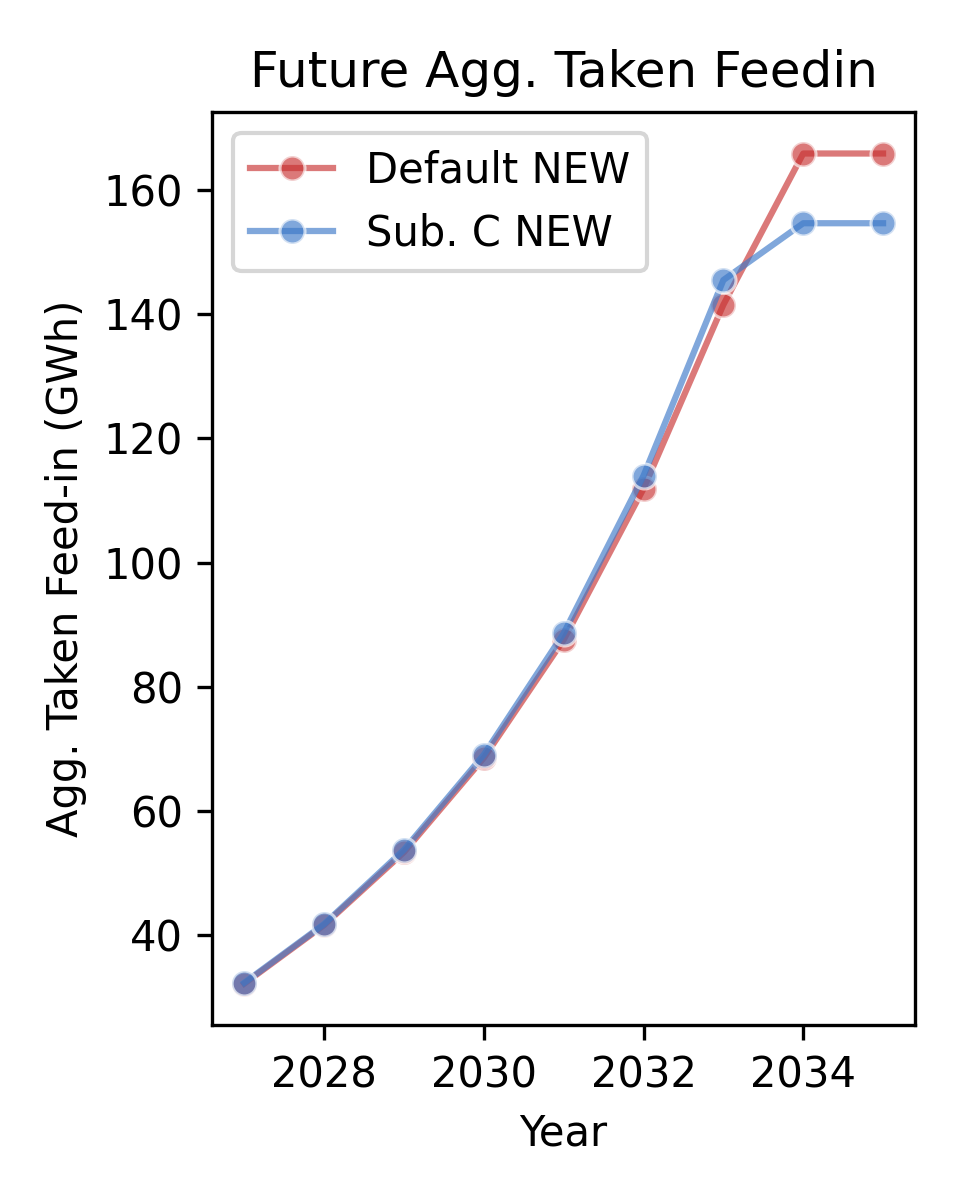
\includegraphics[width=\textwidth]{figures/line_PVproduction_takenfeedin2.png}
\end{minipage}

% \vspace{0.2cm}
{\footnotesize
Linke Grafik zeigt den angepassten, zukünftigen Ausbaupfad (neu mit Startwert auf der historisch verbauten Kapazität in 2023). Netzbedingte Überproduktion tritt erst 2031 auf statt zuvor 2029 (Subsidy C noch später).
% verzögern sich  Durch tieferen Verlauf kann auch länger im Simulationssample zugebaut werden. Dadurch verzögern sich die Kontenkapaz
}
\end{frame}


% -------------------------------------------------------
\begin{frame}[t]{Überproduktion: Schlimmster Tag in den schlimmsten Trafos}
\hypertarget{worstnodesworstweek}{}  
  \centering
  {\footnotesize
  \begin{tabular}{l|rrrrr}
    \toprule
    \textbf{Parameter}
      &  \textcolor[RGB]{200,50,50}{\textbf{751}}
      & \textbf{524}
      & \textbf{754}
      & \textbf{10}
      & \textbf{734} \\
    \midrule
    Peak day
      & \textcolor{black}{17.07.}
      & 17.07.
      & 17.04.
      & 17.07.
      & 17.07. \\
    Total excess feed-in (kWh)
      & \textcolor{black}{6'259.6}
      & 5'424.9
      & 4'215.7
      & 3'751.2
      & 3'192.6 \\
    n h ouses
      & \textcolor{black}{379}
      & 243
      & 283
      & 197
      & 167 \\
    Avg.\ excess feed-in p.\ house (kWh)
      & \textcolor[RGB]{200,50,50}{16.5}
      & 22.3
      & 14.9
      & 19.0
      & 19.1 \\
    Avg.\ remaining netdemand p.\ house (kWh)
      & \textcolor[RGB]{200,50,50}{2.1}
      & 3.2
      & 6.2
      & 4.1
      & 2.2 \\
    \midrule
    Tesla Powerwall (kWh, \cite{tesla2026})  & \textcolor{black}{13.5} & & & &\\
    \bottomrule
  \end{tabular}
  }
  \vspace{0.412cm}

  \begin{columns}[T]
    \begin{column}{0.48\textwidth}
      \centering
        
\includegraphics[width=\textwidth]{figures/hist_avgloss_pEGID_pvalloc_LRG3_max.png}
    \end{column}
    \begin{column}{0.48\textwidth}
      \centering
        
\includegraphics[width=\textwidth]{figures/worstnode_worstweek_pegid_pvalloc_LRG3_max.png}
    \end{column}
  \end{columns}
  
% \vspace{0.1cm}
{\footnotesize
% Linke Grafik zeigt den angepassten Ausbaupfad für die zukünftigen Jahre (neu mit Startwert auf der historisch verbauten Kapazität in 2023). Erste netzbedingte Überproduktion (Excess Feedin) tritt somit erst ca. 2031 statt zuvor 2029. 
% verzögern sich  Durch tieferen Verlauf kann auch länger im Simulationssample zugebaut werden. Dadurch verzögern sich die Kontenkapaz
}
\end{frame}


% -------------------------------------------------------
\begin{frame}[t]{Sensitivitätsanalyse: Halbierung / Verdoppelung Strompreis}
\hypertarget{npv_hists_elecpri}{}

\begin{minipage}{0.322\textwidth}
  \centering
\includegraphics[width=\textwidth]{figures/NPVhist_LRG3_max_31Rp.png}
\end{minipage}\hfill
\begin{minipage}{0.322\textwidth}
  \centering
\includegraphics[width=\textwidth]{figures/NPVhist_LRG3_max_15Rp.png}
\end{minipage}\hfill
\begin{minipage}{0.322\textwidth}
  \centering
\includegraphics[width=\textwidth]{figures/NPVhist_LRG3_max_60Rp.png}
\end{minipage}

\vspace{0.1cm}
{\footnotesize
Grafiken zeigen Histogramm der NPVs aller zukünftigen Installationen bei Strompreis von 31.9,  15 und 60 Rp/kWh. Verschobenen Masse betrifft hauptsächlich Anlagen mit hohem Eingenverbrauch welche (netzdienlicher) zuerst installiert werden. 
}
\end{frame}



%%%%%%%%%%%%%%%%%%%%%%%%%%%%%%%%%%%%%%%%%%%%%%%
\section{Data}

% -------------------------------------------------------
\begin{frame}{Data}

\begin{columns}[t]
\begin{column}{0.48\textwidth}

  \centering\textbf{Summary}\\
  \vspace{0.2cm}
  {\scriptsize
  \setlength{\tabcolsep}{3.5pt}
  \renewcommand{\arraystretch}{1.15}
  \begin{tabular}{l c c c}
    \toprule
    \textbf{Parameter} & \textbf{Sample} & \textbf{Avail.} & \textbf{All CH} \\
    \midrule
    n Municipalities         & 28     & 79      & 2'133     \\
    n All Buildings          & 44'354 & 132'018 & 3'090'962 \\
    n Resid. Houses          & 21'599 & 47'900  & 1'716'194 \\
    n Grid Nodes             & 391    & 1'113   & --        \\
    Inst. Cap. 2024 (MW)     & 20.6   & 79.0    & 2'450.1   \\
    Capacity 2050 (MW)       & 115.6  & 739.5   & 17'313.8  \\
    \bottomrule
  \end{tabular}
  }

\end{column}
\begin{column}{0.48\textwidth}

  \centering\textbf{Data Sources}\\
  \vspace{0.2cm}
  {\scriptsize
  \setlength{\tabcolsep}{3.5pt}
  \renewcommand{\arraystretch}{1.15}
  \begin{tabular}{l l l}
    \toprule
    \textbf{Category} & \textbf{Description} & \textbf{Ref.} \\
    \midrule
    Rooftop Data      & Roof surface, orientation, tilt             & [1]     \\
    Building Data     & Type, heating, prices/tariffs               & [2--5]  \\
    Grid Infra.       & Nodes, connections + capacity               & (NDA)   \\
    Other Data        & Demand, costs, targets, radiation           & [6--9]  \\
    Computing         & HPC cluster for model run                   & [10]    \\
    \bottomrule
  \end{tabular}
  \vspace{0.2cm}
  }

  {\tiny
  \raggedright
  [1]: \cite{solkat2023}\par
  [2--5]: \cite{gwr2025, elec_prod2024, vese_pvtarif2023, elcom2023}\par
  [6--9]: \cite{swissstore2022, energieschweiz2023, bfe_ep2050_2020, meteoblue2023}\par
  [10]: \cite{hpc_scicore2026}\par
  }

\end{column}
\end{columns}
\end{frame}

% %%%%%%%%%%%%%%%%%%%%%%%%%%%%%%%%%%%%%%%%%%%%%%%
% \section{Outlook}

% % -------------------------------------------------------
% \begin{frame}{Conclusion}

%   \begin{block}{Research Contribution}
%     \begin{enumerate}
%       \item \textbf{Problem quantification} $\rightarrow$\textit{Problems will arise in the next couple of years and might scale up fast, dependent on the growth rate of newly installed capacity.}
%       \vspace{0.1cm}
%       \item \textbf{Economic response} $\rightarrow$ \textit{Simple subsidy adjustments might delay grid congestion by a few years and could be even as good as a social planner's allocation.}
%     \end{enumerate}
%   \end{block}

%   \textbf{Outlook}
%   \begin{itemize}
%     \item Post calculation: battery capacity for "worst week" in "worst node" (in progress).
%     \item Cost comparison of subsidy spending to grid reinforcements in most affected nodes.
%   \end{itemize}

%   \textbf{Postponed}
%   \begin{itemize}
%     \item Add battery investment and battery usage to the model
%     \begin{itemize}
%       \item Optimized for household consumption vs.\ grid serving (quasi-obligatory for PV installations)
%     \end{itemize}
%   \end{itemize}

% \end{frame}



%%%%%%%%%%%%%%%%%%%%%%%%%%%%%%%%%%%%%%%%%%%%%%%
\section{Model}

% % -------------------------------------------------------
% \begin{frame}{Model Simulation - 3 Agents}
% \hypertarget{mod_structure_agents}{}

% \begin{columns}[t]

% \begin{column}{0.49\textwidth}
%   \only<1->{\textcolor[RGB]{128,0,128}{Production}
%   \vspace{-0.0961cm}
%   \begin{itemize}
%     \item Roof partitions and radiation time series yield production potential.
%     \vspace{-0.0961cm} 
%     \item Calibrated random forest assigns installation size \hyperlink{appendix_randomforest_scatterplot}{\beamerreturnbutton{App. RFR}}.
%   \end{itemize}}
%   \only<2->{\textcolor[RGB]{204,85,0}{Demand} ($\rightarrow$ \textcolor[RGB]{0,70,127}{Feed-in})
%   \vspace{-0.0961cm}
%   \begin{itemize}
%     \item 6 Archetype profiles scaled by living area (\cite{swissstore2022}).
%     \vspace{-0.0961cm}
%     \item Heat pumps: Scaling up winter months.
%   \end{itemize}}
%   \only<3->{\textcolor{unibasgreydark}{Investments}
%   \vspace{-0.0961cm}
%   \begin{itemize}
%     \item General cost assumption of PV calculator (\cite{energieschweiz2023} \hyperlink{appendix_cost_function}{\beamerreturnbutton{App. Cost}})
%   \end{itemize}
%   % $\rightarrow NPV_{i} = -Inv_{i} + \sum_{t}^{25}\frac{SelfCons_{i,t} P_{elec,t} + Feedin_{i,t} P_{pv,t}}{(1+r)^t}$}
%   }
%   \vspace{0.35cm}
%   \only<4->{$\rightarrow NPV_{i} = -Inv_{i} + \sum_{t}^{25}\frac{SelfCons_{i,t} + Feedin_{i,t} }{(1+r)^t}$
%   }
%   \vfill
% \end{column}

% \begin{column}{0.49\textwidth}
%   \begin{figure}
%     \centering
%     
\includegraphics[width=0.481\linewidth]{SSES_StGallen/figures/EGID_solkat_example.png}
%   \end{figure}
%   \vspace{-0.2cm}
%   \begin{figure}
%     \centering
%     \only<1>{
\includegraphics[width=0.91\linewidth]{SSES_StGallen/figures/plot_EGID_HOY_pvprod.png}}%
%     \only<2>{
\includegraphics[width=0.91\linewidth]{SSES_StGallen/figures/plot_EGID_HOY_pvprod_demand.png}}%
%     \only<3->{
\includegraphics[width=0.91\linewidth]{SSES_StGallen/figures/plot_EGID_HOY_pvprod_demand_feedin.png}}%
%   \end{figure}
% \end{column}

% \end{columns}
% \end{frame}

% % -------------------------------------------------------
% \begin{frame}{Allocation Process}
% \hypertarget{mod_allocation_process}{}

% \begin{columns}[t]

% \begin{column}{0.49\textwidth}
%   \textbf{Allocation process}
%   \begin{itemize}
%     \item NPV defines installation "order" (similar to \cite{arguello2018},
%       \hyperlink{appendix_npv_hist_sensitivity}{\beamerreturnbutton{App. NPV}}).
%     \item Scaled, adjusted, annual ``construction budget'' (\cite{bfe_ep2050_2020}) until 2050.
%   \end{itemize}

%   \vspace{-0.2cm}
%   \begin{figure}
%     \centering
%     
\includegraphics[width=0.84\linewidth]{SSES_StGallen/figures/NPVhist_LRG3_max.png}
%   \end{figure}
% \end{column}

% \begin{column}{0.49\textwidth}
%   \textbf{Subsidy adjustment}
%   \begin{itemize}
%     \item Subsidy budget given to operator (transparent criteria)
%     \item 3 types (A: roof orientation, B: grid specific, C: combination)
%   \end{itemize}

%   \[
%     \rightarrow NPV_{i,X} = NPV_{i} + S_{i,X} - R_{i,X}
%   \]

%   \vspace{0.3cm}
%   \centering
%   \footnotesize
%   \begin{tabular}{|l| c c c c|}
%     \hline
%     & $S=0$ & 4000 & 6000 & 8000 \\
%     \hline
%     $R=0$ & BU & \cellcolor{scenA_table} & \cellcolor{scenA_table} A & \cellcolor{scenA_table} \\
%     4000  & \cellcolor{scenB_table} & \cellcolor{scenC_table} & \cellcolor{scenC_table} & \cellcolor{scenC_table} \\
%     6000  & \cellcolor{scenB_table} B & \cellcolor{scenC_table} & \cellcolor{scenC_table} C & \cellcolor{scenC_table} \\
%     8000  & \cellcolor{scenB_table} & \cellcolor{scenC_table} & \cellcolor{scenC_table} & \cellcolor{scenC_table} \\
%     \hline
%   \end{tabular}
% \end{column}

% \end{columns}
% \end{frame}


%%%%%%%%%%%%%%%%%%%%%%%%%%%%%%%%%%%%%%%%%%%%%%%
\section*{Appendix}
% \appendix
% \backupbegin

% % -------------------------------------------------------
% \begin{frame}{Appendix: NPV Sensitivity --- Electricity Prices}
% \hypertarget{appendix_npv_hist_sensitivity}{}
% \begin{minipage}{0.48\textwidth}
%   \centering\includegraphics[width=\textwidth]{SSES_StGallen/figures/pvalloc_LRG3_max_elecpri15RP_npv_df_hist.png}
% \end{minipage}\hfill
% \begin{minipage}{0.48\textwidth}
%   \centering\includegraphics[width=\textwidth]{SSES_StGallen/figures/pvalloc_LRG3_max_elecpri60RP_npv_df_hist.png}
% \end{minipage}
% \centering
% \hyperlink{mod_allocation_process}{\beamerreturnbutton{back}}
% \end{frame}

% % -------------------------------------------------------
% \begin{frame}{Appendix: High Spatial Resolution at Large Scale}
% \begin{minipage}{0.323\textwidth}
%   \centering
\includegraphics[width=\textwidth]{SSES_StGallen/figures/wp_topo_roof_solkat_1_3.png}
% \end{minipage}\hfill
% \begin{minipage}{0.323\textwidth}
%   \centering
\includegraphics[width=\textwidth]{SSES_StGallen/figures/wp_topo_DSO_example_1_3.png}
% \end{minipage}\hfill
% \begin{minipage}{0.323\textwidth}
%   \centering
\includegraphics[width=\textwidth]{SSES_StGallen/figures/wp_topo_DSO_grid_large_example_1_3.png}
% \end{minipage}
% \end{frame}

% % -------------------------------------------------------
% \begin{frame}{}
% \begin{minipage}{0.479\textwidth}
%   Business as Usual\\
%   \centering
%   
\includegraphics[width=1.0\textwidth]{paper_publication/SSES_StGallen/hist_contcharact_newinst_bu_pvalloc_LRG3_max.png}
%   \vspace{-0.311cm}
%   \begin{minipage}{0.49\textwidth}
%     \centering\makebox[0pt][c]{
\includegraphics[width=1.05\textwidth]{SSES_StGallen/figures/line_catgcharact_newinst_bu_pvalloc_LRG3_max_GKLAS.png}}
%   \end{minipage}\hfill
%   \begin{minipage}{0.49\textwidth}
%     \centering\makebox[0pt][c]{
\includegraphics[width=1.05\textwidth]{SSES_StGallen/figures/line_catgcharact_newinst_bu_pvalloc_LRG3_max_heatpump_TF.png}}
%   \end{minipage}
%   \vspace{-0.311cm}
%   \begin{minipage}{0.49\textwidth}
%     \centering\makebox[0pt][c]{
\includegraphics[width=1.05\textwidth]{SSES_StGallen/figures/line_catgcharact_newinst_bu_pvalloc_LRG3_max_are_typ.png}}
%   \end{minipage}\hfill
%   \begin{minipage}{0.49\textwidth}
%     \centering\makebox[0pt][c]{
\includegraphics[width=1.05\textwidth]{SSES_StGallen/figures/line_catgcharact_newinst_bu_pvalloc_LRG3_max_filter_tag.png}}
%   \end{minipage}
% \end{minipage}
% \begin{minipage}{0.479\textwidth}
%   Subsidy B\\
%   \centering
%   
\includegraphics[width=1.0\textwidth]{paper_publication/SSES_StGallen/hist_contcharact_newinst_bu_pvalloc_LRG3_max.png}
%   \vspace{-0.311cm}
%   \begin{minipage}{0.49\textwidth}
%     \centering\makebox[0pt][c]{
\includegraphics[width=1.05\textwidth]{SSES_StGallen/figures/line_catgcharact_newinst_bu_pvalloc_LRG3_max_sBs0p8_GKLAS.png}}
%   \end{minipage}\hfill
%   \begin{minipage}{0.49\textwidth}
%     \centering\makebox[0pt][c]{
\includegraphics[width=1.05\textwidth]{SSES_StGallen/figures/line_catgcharact_newinst_bu_pvalloc_LRG3_max_sBs0p8_heatpump_TF.png}}
%   \end{minipage}
%   \vspace{-0.311cm}
%   \begin{minipage}{0.49\textwidth}
%     \centering\makebox[0pt][c]{
\includegraphics[width=1.05\textwidth]{SSES_StGallen/figures/line_catgcharact_newinst_bu_pvalloc_LRG3_max_sBs0p8_are_typ.png}}
%   \end{minipage}\hfill
%   \begin{minipage}{0.49\textwidth}
%     \centering\makebox[0pt][c]{
\includegraphics[width=1.05\textwidth]{SSES_StGallen/figures/line_catgcharact_newinst_bu_pvalloc_LRG3_max_sBs0p8_filter_tag.png}}
%   \end{minipage}
% \end{minipage}
% \end{frame}

% % -------------------------------------------------------
% \begin{frame}{Appendix: Model Grid Analysis EP2050+}
% \hypertarget{appendix_model_grid_analysis}{}
% \vspace{-\baselineskip}
% \begin{figure}
%   \centering
%   
\includegraphics[width=0.8\textwidth]{SSES_StGallen/figures/bfe_ep2050_netz_MNA_notitle.PNG}
% \end{figure}
% \vspace{-\baselineskip}
% \small\centering
% \textit{Comparison between the real (left) and homogeneous model assumed grid topology \cite{bfe_ep2050_netz2022}}
% \hyperlink{back}{\beamerreturnbutton{Literature}}
% \end{frame}

% % -------------------------------------------------------
% \begin{frame}{Appendix: Calibrated Random Forest}
% \hypertarget{appendix_randomforest_scatterplot}{}
% \vspace{-\baselineskip}
% \begin{figure}
%   \centering
%   
\includegraphics[width=0.56\textwidth]{SSES_StGallen/figures/calib_rfr2_predvsactual.png}
% \end{figure}
% \vspace{-\baselineskip}
% \small\centering
% \textit{Scatterplot for actual and predicted installation sizes (incl.\ 45° diagonal) of calibrated random forest regression on 61270 Swiss houses with a PV installation, between 20 to 70 percent of available roof partition used.}
% \hyperlink{mod_structure_agents}{\beamerreturnbutton{back}}
% \end{frame}

% % -------------------------------------------------------
% \begin{frame}{Appendix: Interpolated Cost Function}
% \hypertarget{appendix_cost_function}{}
% \vspace{-\baselineskip}
% \begin{figure}
%   \centering
%   
\includegraphics[width=0.56\textwidth]{SSES_StGallen/figures/pvinstcost_table.png}
% \end{figure}
% \vspace{-\baselineskip}
% \small\centering
% \textit{Interpolation approximation function (green, only on small scale installations) based on cost assumptions in the technical model appendix of energieschweiz.}
% \hyperlink{mod_structure_agents}{\beamerreturnbutton{back}}
% \end{frame}

% % -------------------------------------------------------
% \begin{frame}{Appendix: RES Targets 2050 Switzerland}
% \hypertarget{appendix_res_targets}{}
% \vspace{-\baselineskip}
% \begin{figure}
%   \centering
%   
\includegraphics[width=0.56\textwidth]{SSES_StGallen/figures/eth_summerschool_scenario_agg_notitle.png}
% \end{figure}
% \vspace{-\baselineskip}
% \hyperlink{motivation_relevance}{\beamerreturnbutton{back}}
% \end{frame}


%%%%%%%%%%%%%%%%%%%%%%%%%%%%%%%%%%%%%%%%%%%%%%%
\section*{Bibliography}
\renewcommand{\bibfont}{\footnotesize}
\begin{frame}[allowframebreaks]{References}
  \printbibliography
\end{frame}

\end{document}
